\section{Sequential Modeling}

	\begin{figure}[htbp]
		\centering
		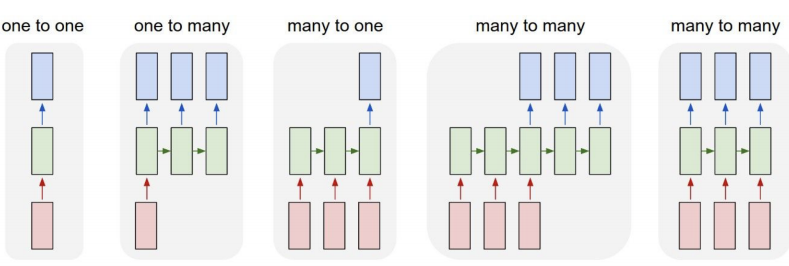
\includegraphics[scale=0.65]{figures/rnn-seqdata.png}
		\caption{各种输入输出方式}
	\end{figure}

	我们之前的网络,都是one-to-one,一个输入,一个输出.
	
	one-to-many:例如看图说话, Image Captioning, image$\rightarrow$sequence of words
	
	many-to-one:例如动作预测.
	
	many-to-many:例如video captioning, 或者 Video classification on frame level 可以看作是沿着时间维度的 action segmentation.

	此外还有offline和online的处理.前者全部看完,后者边看边输出.
	
	\subsection{Recurrent Neural Network (RNN)}
	
	还有 recursive NN, 但是不常用

	Key point: RNNs有一个在处理序列时会更新的 hidden state, 就是 $h$

	\begin{figure}[htbp]
		\centering
		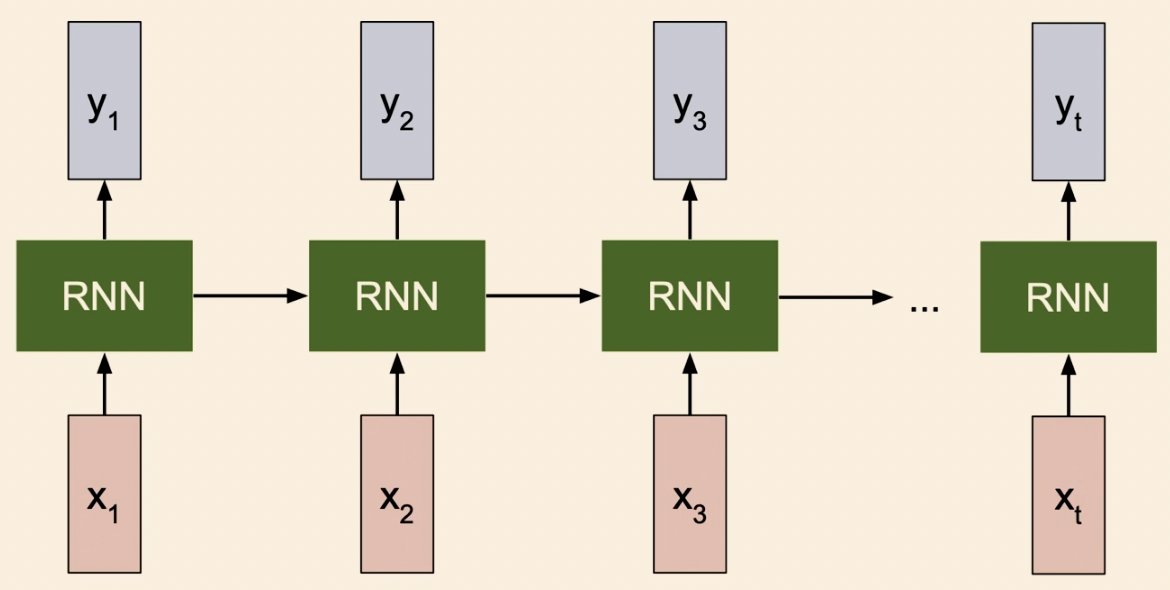
\includegraphics[scale=0.3]{figures/rnn.png}
		\caption{RNN: 典型的 many-to-many}
	\end{figure}

	值得注意的是, RNN 的架构很灵活, 可以容易改变输出输出从而变成 many-to-one, one-to-many 等等

	\begin{equation}
		\begin{cases}
			h_t = f_W\xk{h_{t-1}, x_t}
			\\
			y_t = f_{W_{hy}}\xk{h_t}
		\end{cases}
	\end{equation}

	输出的 $y_t$ 作为一个 decoder, 在需要输出结果的时候输出,否则不输出

	最开始的 $h_0$ 一般是全零的, 也可以是随机的,只要一样就行

	\subsection{Vanilla RNN}

	最初始的RNN

	P.S. 叫做 vanilla 是因为它是最原始的

	\begin{equation}
		\begin{cases}
			h_t = \tanh\xk{W_{hh}h_{t-1} + W_{xh}x_t}
			\\
			y_t = W_{hy}^*h_t
		\end{cases}
	\end{equation}
	
	计算图,各个方向流向W:
	
	\begin{figure}[htbp]
		\centering
		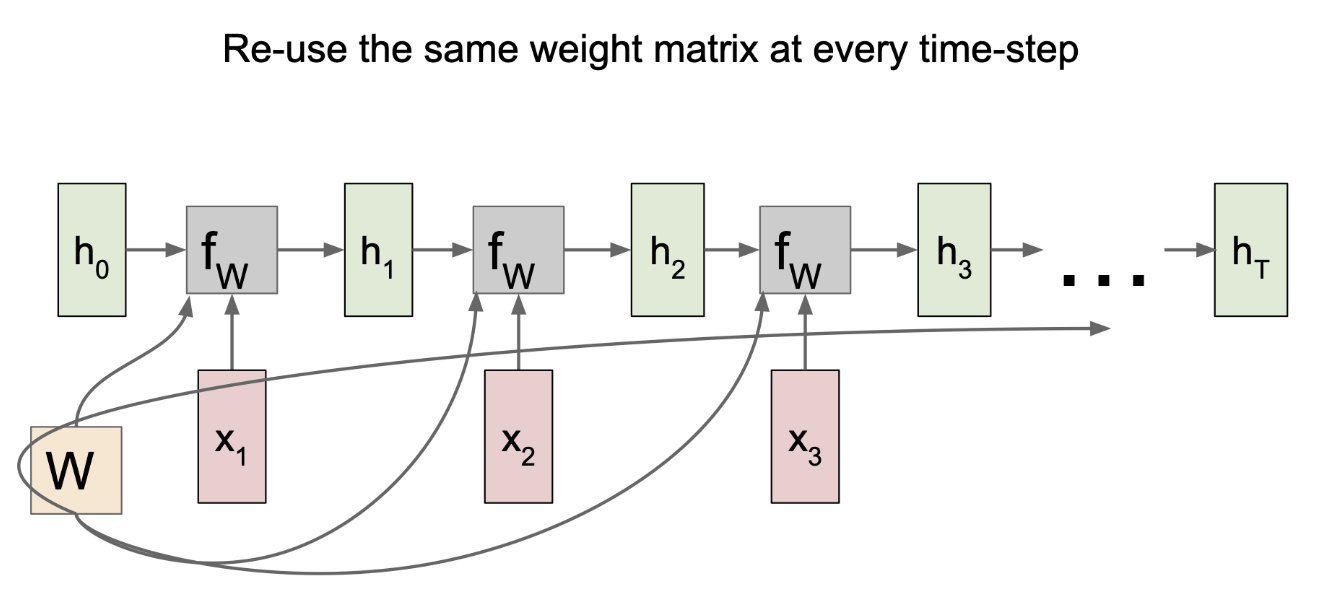
\includegraphics[scale=0.2]{figures/vanilla_rnn.png}
		\caption{Vanilla RNN Computational Graph}
	\end{figure}
	
	\textbf{\\Characer-Level Language Model}

	\begin{figure}[htbp]
		\centering
		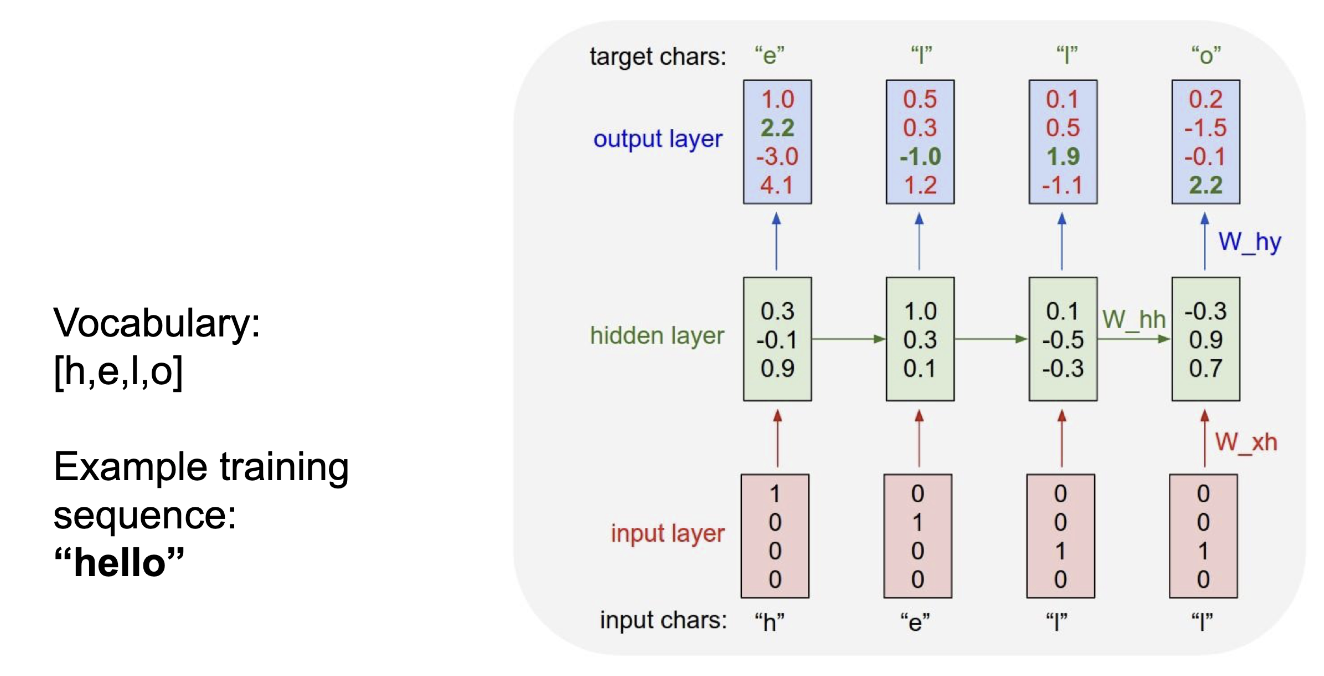
\includegraphics[scale=0.2]{figures/word_model.png}
		\caption{Characer-Level Language Model}
	\end{figure}

	先考虑简单的模型, character-level language model, 有限集合的字符, 
	比如英文26个字母, 逗号, 句号等等

	BP时,不同位置的W被loss调用了不同次.这个操作开销极大.

	\begin{figure}[htbp]
		\centering
		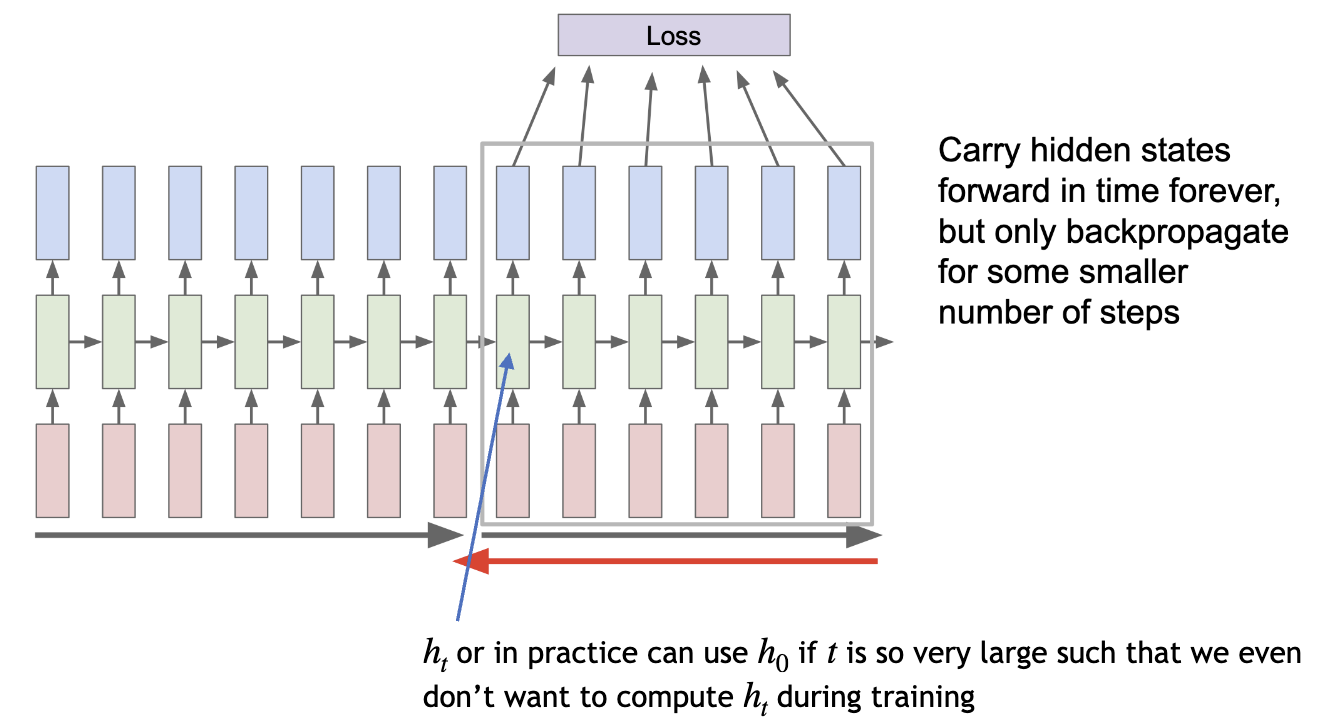
\includegraphics[scale=0.2]{figures/truncate_bp.png}
		\caption{Truncated BP}
	\end{figure}
	
	解决方法:truncated BP截断回传.比如FP时是从0到t,BP只算从t到t-6.

	这个window length是sequence length

	\textbf{\\Why share weight?} 
	
	就像CNN一样,我们希望词特征是等变的.同一句话,在文章中的不同位置,应该具有相同的特征.

	\textbf{\\Different Sampling Strategies}

	\begin{itemize}
		\item Greedy sampling: 总是取最高概率的token
		
		问题:确定性,只能在给定初始标记和隐藏状态的情况下生成一个序列

		\item Weighted sampling: 根据预测的概率分布采样下一个标记
		
		优点:可以生成多样的序列
		
		问题:可能会意外获得错误的标记并造成生成过程的错误
		
		\item Exhaustive Search
		\[
		\begin{aligned}P(y|x)&=P(y_1|x)P(y_2|y_1,x)P(y_3|y_1,y_2,x)\ldots,P(y_T|y_1,\ldots,y_{T-1},x)\\&=\prod_{t=1}^TP(y_t|y_1,\ldots,y_{t-1},x)\end{aligned}
		\]

		\item Beam Search: 最有可能的前K个,下次从KV结果中选择K个最有可能的
	\end{itemize}
	
	实际上将h和x结合的时候,常常先将x进行embedding, W(h,x) $\rightarrow$ W(h, g(x)).
	比如,hidden layer可能之后512维,但是输入如果是词向量,那么可能有几万维,
	非常不均衡.因此将embedding到合适的维度.此外,word embedding已经有现成的处理.
	
	RNN在长程记忆里会出现问题, $\Delta T$一般被称为sequence length,如果过短则相关性不强,过长则cost too much.
	
	\subsection{RNN tradeoff}
	\begin{itemize}
		\item RNN 优点:
		\begin {itemize}
			\item 可以处理任何长度的输入
			\item 步骤 t 的计算(理论上)可以使用许多步之前的信息
			\item 模型大小不会因输入更长而增加
			\item 在每个时间步上应用相同的权重,因此输入处理方式是等变的
		\end{itemize}
		\item RNN 缺点:
		\begin{itemize}
			\item 循环计算很慢
			\item 在实践中,很难从许多步骤前获取信息
		\end{itemize}
	\end{itemize}

	\subsection{Multilayer RNNs}
	\begin{figure}[htbp]
		\centering
		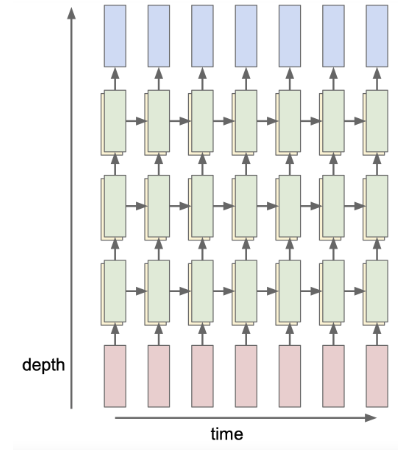
\includegraphics[scale=0.35]{figures/multilayer_rnn.png}
		\caption{Multilayer RNN}
	\end{figure}

	增强RNN非线性的能力
	
	\subsection{Vanilla RNN Gradient Flow}

	\begin{figure}[H]
		\centering
		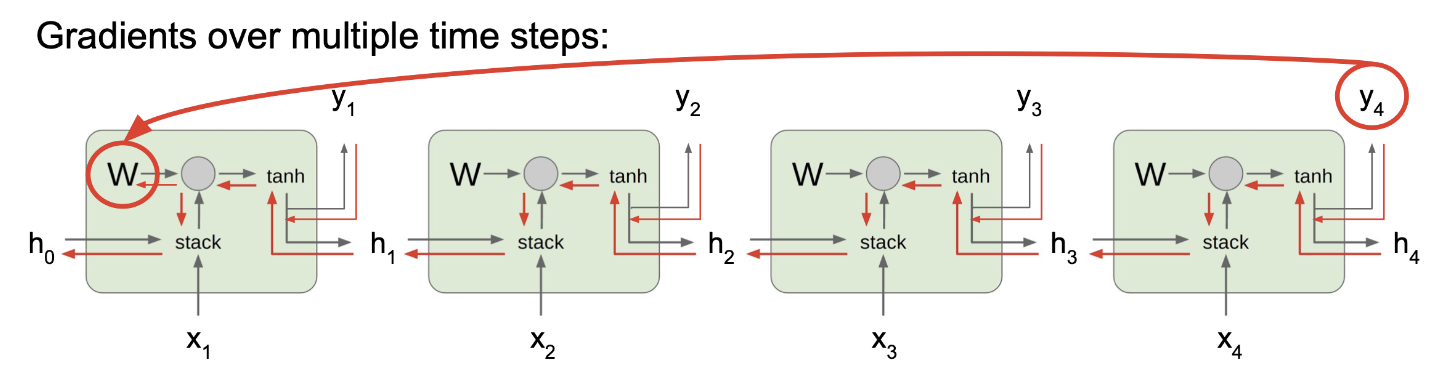
\includegraphics[scale=0.3]{figures/RNN_grad_van.png}
		\caption{Vanilla RNN Gradient Flow}
	\end{figure}

	\[
	\begin{aligned}
		h_{t}& =\tanh(W_{hh}h_{t-1}+W_{xh}x_{t})  \\
		&=\tanh\left(\begin{pmatrix}W_{hh}&W_{hx}\end{pmatrix}\begin{pmatrix}h_{t-1}\\x_t\end{pmatrix}\right) \\
		&=\tanh\left(W\begin{pmatrix}h_{t-1}\\x_t\end{pmatrix}\right)
		\end{aligned}	
	\]
	
	tanh的梯度恒小于1,梯度消失:

	\[
		\frac{\partial h_t}{\partial h_{t-1}}=tanh^{\prime}(W_{hh}h_{t-1}+W_{xh}x_t)W_{hh}	
	\]

	\[
		\frac{\partial L_T}{\partial W}=\frac{\partial L_T}{\partial h_T}\frac{\partial h_t}{\partial h_{t-1}}\ldots\frac{\partial h_1}{\partial W}=\frac{\partial L_T}{\partial h_T}(\prod_{t=2}^T\frac{\partial h_t}{\partial h_{t-1}})\frac{\partial h_1}{\partial W}	
	\]

	远处的梯度信号丢失了, 因为它比近处的梯度信号小得多, 模型权重仅针对近期进行更新, 而非长期
	
	\textbf{gradient clipping}对于exploding grad有一定作用, 但是解决不了 vanishing gradient 的问题.必须Change RNN architecture
	
	\subsection{LSTM}

	\begin{figure}[H]
		\centering
		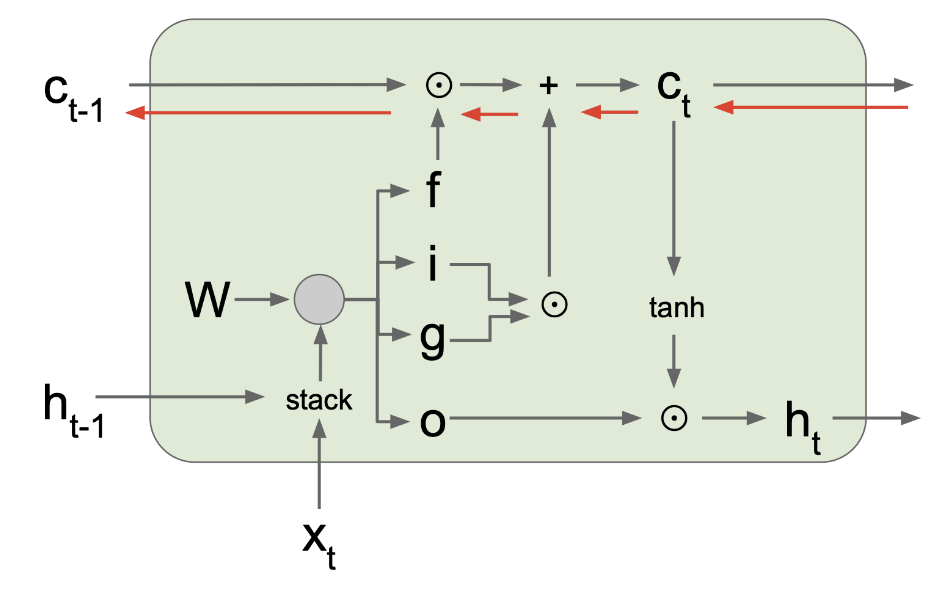
\includegraphics[scale=0.2]{figures/lstm_grad_flow.png}
		\caption{LSTM Gradient Flow}
	\end{figure}

	\[
	\begin{aligned}
		\begin{pmatrix}i\\f\\o\\g\end{pmatrix}& =\begin{pmatrix}\sigma\\\sigma\\\sigma\\\tanh\end{pmatrix}W\begin{pmatrix}h_{t-1}\\x_t\end{pmatrix}  \\
		&c_{t} =f\odot c_{t-1}+i\odot g  \\
		&h_{t} =o\odot\tanh(c_t) 
	\end{aligned}
	\]

	\begin{itemize}
		\item i: Input gate, Whether to write to cell
		\item f: Forget gate. Whether to erase cell
		\item o: Output gate, How much to reveal cell
		\item g: Gate gate (?), How much to write to cell
	\end{itemize}
	
	cell state是long-term memory.我们知道对于普通的tanh,往01之间映射,那么$h_t$和很早之前的$h_i$之间的联系就比较微弱了.
	而LSTM中的c则一直把信息保留(f也是经过sigmoid激活的,在01之间,可以选择记住或者遗忘),最后h将c进行处理.
	
	核心结构:old info和new info的加和.若f=1,则就是skiplink.换言之c之间有梯度的旁路.

	因为c是旁路,梯度可以直接流过来

	\textbf{\\Do LSTMs Solve the Vanishing Gradient Problem?}

	不能保证. 但是这种skip link的结构可以缓解这个问题.

	Long term dependencies 的问题得到了很好的解决

	\subsection{Gated Recurrent Unit (GRU)}

	\[
	\begin{aligned}
		&r_{t} =\sigma(W_{xr}x_t+W_{hr}h_{t-1}+b_r)  \\
		&z_{t} =\sigma(W_{xz}x_t+W_{hz}h_{t-1}+b_z)  \\
		&\tilde{h}_{t} =\tanh(W_{xh}x_t+W_{hh}(r_t\odot h_{t-1})+b_h)  \\
		&h_t =z_t\odot h_{t-1}+(1-z_t)\odot\tilde{h}_t 
	\end{aligned}	
	\]

	性能不输LSTM, 有的时候还更好

	了解即可

	\subsection{Summary}

	LSTM是一种RNN, 所有Sequencial Model都是RNN, 只是不是vanilla RNN